\chapter{Ricerca framework adatto}
\label{sec:ricerca_framework}

Una volta esaminata l'implementazione attuale e identificati i suoi principali
problemi nel capitolo precedente, è stato deciso di utilizzare un approccio DRY.
L'acronimo DRY, Don't Repeat Yourself, si riferisce al principio in Computer
Science in cui "Ogni conoscenza deve avere una rappresentazione unica, univoca e
autorevole all’interno di un sistema" descritto in \texttt{The Pragmatic
Programmer}\cite{thomas2019pragmatic}. In questo caso ne viene esteso il
significato per riferirsi all'utilizzo di framework esterni testati e che hanno
dimostrato di funzionare.

\section{Prerequisiti}
\label{sec:prerequisiti}

Viene fatta ora un'analisi esaustiva dei prerequisiti da considerare e valutare durante
il processo di ricerca \ref{sec:candidates} e scelta \ref{sec:airflow} del framework
che verrà usato per sostituire l'attuale implementazione. Si individuano i
prerequisiti fondamentali riportati di seguito.

\subsection{Utilizzo efficiente delle risorse}
\label{sub:resource_usage}

Primo prerequisito fondamentale è la possibilità di sfruttare completamente le risorse
a disposizione. Questo significa che bisognerà inizialmente favorire la
scalabilità verticale del sistema, in questo modo è possibile partire da un sistema
più semplice che verrà esteso in seguito. Scalare verticalmente comporta creare
una macchina unica più potente e risparmiare nel complesso risorse, in quanto l'overhead
del sistema operativo è presente soltanto una volta e un core può effettivamente
eseguire più task alla volta sfruttando il multithreading.

\subsection{Definizione dipendenze tramite DAG}
\label{sub:deps_definition}

Come visto nella sezione \ref{sub:robots}, vengono definite delle dipendenze tra
fasi. Uno dei prerequisiti fondamentali è la possibilità di definire in modo
esplicito grafi di dipendenze, non dovendo quindi pensare per ogni fase quali devono
essere quelle che la precedono o la seguono. Sarebbe ideale un'implementazione
analoga a quella riportata nel codice \ref{lst:dag-example} e renderizzata in
figura \ref{fig:dag-example}.

\begin{figure}[htbp]
  \centering
  \begin{minipage}{0.45\textwidth}
    \centering
    \lstinputlisting[language=Python, caption=Esempio di definizione di DAG in Airflow,
    label=lst:dag-example ]{listings/dag-example.py}
  \end{minipage}
  \hfill
  \begin{minipage}{0.45\textwidth}
    \centering
    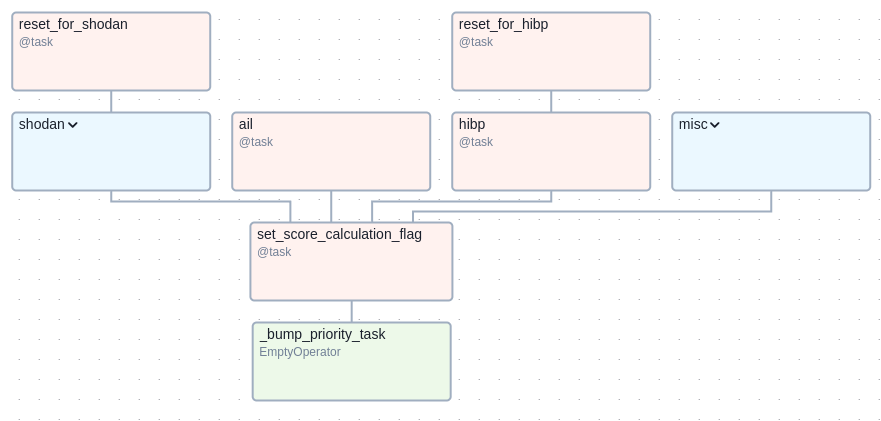
\includegraphics[width=\textwidth]{images/dag-example.png}
    \caption{Esempio di renderizzazione del DAG}
    \label{fig:dag-example}
  \end{minipage}
\end{figure}

\subsection{Compatibilità con Python}
\label{sub:python_compatibility}

Il linguaggio di programmazione principale, in cui è scritta la parte di collezione
e serializzazione dei dati, è Python. Questo significa che gran parte delle fasi
eseguite dalle macchine Robot possono essere utilizzate nella nuova implementazione
senza cambiamenti radicali. Data la natura della maggior parte delle task, che svolgendo
ricerche OSINT, vengono eseguite molte richieste di rete. Ciò significa che, per
la maggior parte del tempo, il processo resta in attesa di una risposta da un server
remoto (I/O intensive) e non esegue operazioni computazionalmente pesanti (CPU
intensive). Per questo motivo utilizzare un linguaggio di programmazione più
performante non aumenterebbe molto le prestazioni e aggiungerebbe soltanto
complessità nel tradurre le implementazioni attuali e gestire codice in un
linguaggio poco conosciuto dal team.

Un'altra caratteristica fondamentale e correlata è la possibilità di definire le
task in modo programmatico, in modo da appunto riutilizzare il codice già presente
e funzionante.

\subsection{Scalabilità orizzontale}
\label{sub:scalable}

Espandendo quanto descritto al requisito \ref{sub:resource_usage}, potrebbe presentarsi
la necessità di scalare e utilizzare più risorse di quelle messe a disposizione dall'infrastruttura
sottostante. Questo problema può essere risolto utilizzare un approccio di
scalabilità orizzontale. Il framework selezionato deve quindi offrire la possibilità
di funzionare su cluster in modo relativamente semplice e veloce, idealmente
utilizzando soluzioni ben conosciute quali Kubernetes\footnote{\url{https://kubernetes.io/}}.

\subsection{Open source, Manutenzione e Documentazione}
\label{sub:open_source}

Prima di valutare strumenti offerti da altre aziende come prodotti a pagamento, è
opportuno valutare la presenza di eventuali strumenti Open source o disponibili gratuitamente.
In ambito Open source bisogna prestare particolare attenzione tre aspetti chiave:
la manutenzione, ovvero quanto attivo è il progetto e quanto velocemente vengono
risolti bug e implementate nuove funzionalità; il supporto, ovvero quanto è
attiva la comunità attorno al progetto per chiedere aiuto in caso di problemi o
difficoltà nell'utilizzo del framework; completezza e chiarezza della documentazione,
fondamentale per utilizzare in modo efficiente tutte le funzionalità del
software in questione.

\subsection{Isolabilità}
\label{sub:isolation}

Alcune fasi implementate all'interno di SATAYO necessitano di un ambiente isolato
per eseguire correttamente. Esempio pratico di questo requisito potrebbe essere
l'utilizzo di una VPN, che forza tutto il traffico del sistema ad uscire attraverso
di essa; questo non permetterebbe a determinate altre fasi di comunicare
correttamente con il server remoto a cui si appoggiano. Analogamente se una determinata
fase utilizza un software Open source di dubbia sicurezza, o con dipendenze
molto vecchie che andrebbero in conflitto con il resto del sistema, è opportuno che
vengano eseguite le fasi all'interno di sandbox che ne limitino le capacità.

\subsection{Monitorabilità}
\label{sub:monitorable}

Ultimo requisito fondamentale è la possibilità di poter monitorare a fondo lo
stato del sistema, ma soprattutto lo stato delle singole fasi che sono in esecuzione.
Più specificatamente è necessario avere una visione molto dettagliata della
parte di schedulazione implementata dal framework, il quale deve mettere a disposizione
metriche collezionabili da sistemi di monitoraggio quali Neteye\cite{neteye} o
Prometheus\footnote{\url{https://prometheus.io/}}.

Per quanto riguarda il collezionamento dei log di esecuzione delle fasi, deve
esserci un metodo standardizzato per produrli in modo tale che possano essere
collezionati da sistemi di collezionamento e indicizzazione come Elasticsearch\footnote{\url{https://www.elastic.co/elasticsearch}}.

\section{Soluzioni candidate}
\label{sec:candidates}

Durante l'attività di ricerca sono stati individuate più soluzioni e framework
che rispettavano alcuni o tutti i requisiti definiti nella sezione precedente. Di
seguito sono riportate le caratteristiche dei candidati più interessanti che sono
stati valutati per la scelta finale, la tabella \ref{table:requisites} riporta
una visualizzazione di tutti i requisiti per ogni framework.

\begin{itemize}
  \item \textbf{multithreading nativo di Python:} prima possibile soluzione, è stata
    immediatamente scartata in quanto rispetta solo il requisito \ref{sub:resource_usage}
    (e \ref{sub:python_compatibility}. Nonostante ciò è risultata molto utile per
    individuare correttamente il requisito \ref{sub:open_source};

  \item \textbf{Celery\footnote{\url{https://docs.celeryq.dev/en/stable/}}:} è
    il primo framework effettivo analizzato come possibile opzione, dalla documentazione
    ufficiale "Celery è un sistema distribuito semplice, flessibile e affidabile
    per elaborare grandi quantità di messaggi, fornendo al tempo stesso alle
    operazioni gli strumenti necessari per mantenere tale sistema". Data questa
    definizione Celery sembra un ottimo candidato, soddisfa pienamente i requisiti:
    \ref{sub:resource_usage} in quanto un nodo worker può sfruttare al meglio le
    risorse eseguendo più fasi in diversi sottoprocessi; \ref{sub:python_compatibility}
    perché scritto interamente in Python e completamente compatibile con esso;
    \ref{sub:open_source} in quanto il progetto è molto grande e mantenuto. Contrariamente
    in Celery non esiste un modo conciso di definire dipendenze tramite DAG,
    \ref{sub:deps_definition}. Esiste la possibilità di scalare orizzontalmente come
    richiesto da \ref{sub:scalable} aggiungendo nodi worker al sistema, bisogna
    però gestirli manualmente e non può essere gestito con piattaforme pre
    esistenti quali Kubernetes. In fine rispetta parzialmente anche il requisito
    \ref{sub:isolation} in quanto nonostante non ci sia un metodo nativo di implementarlo,
    si possono creare più worker in ambienti dedicati diversi, ed eseguire determinate
    task con requisiti particolari in quest'ultimi.

  \item \textbf{Luigi\footnote{\url{https://github.com/spotify/luigi}}:} è un
    pacchetto Python che serve per "costruire pipeline complesse di lavori batch"
    come riportato nella documentazione del progetto. Purtroppo per questo caso d'uso
    però Luigi è troppo semplice e limitante, in quanto come Celery non supporta
    la definizione esplicita di DAG \ref{sub:deps_definition}. Inoltre non permette
    la scalabilità orizzontale \ref{sub:scalable}, né l'isolabilità
    \ref{sub:isolation}; ha una documentazione alquanto limitata e non mette a disposizione
    molte metriche per il monitoraggio.

  \item \textbf{Apache Airflow\cite{airflow}:} come descritto nella pagina
    principale del progetto, "Airflow è una piattaforma creata dalla community
    per creare, pianificare e monitorare in modo programmatico i flussi di lavoro",
    rispetta tutti i requisiti descritti nella sezione \ref{sec:prerequisiti} ed
    è stato scelto come core della nuova implementazione. Verrà descritto più
    nel dettaglio come questo framework ha soddisfatto i requisiti imposti nella
    sezione \ref{sec:airflow}.
\end{itemize}

\begin{table}[htbp]
  \begin{center}
    \renewcommand{\arraystretch}{1.5}
    \begin{tabular}{|>{\centering\arraybackslash}m{6cm}|>{\centering\arraybackslash}m{3cm}|c|c|c|}
      \hline
      \textbf{Requisito}                 & \textbf{multithreading nativo} & \textbf{Luigi} & \textbf{Celery} & \textbf{Apache Airflow} \\
      \hline
      \nameref{sub:resource_usage}       & \cmark                         & \cmark         & \cmark          & \cmark                  \\
      \hline
      \nameref{sub:deps_definition}      & \xmark                         & \xmark         & \xmark          & \cmark                  \\
      \hline
      \nameref{sub:python_compatibility} & \cmark                         & \cmark         & \cmark          & \cmark                  \\
      \hline
      \nameref{sub:scalable}             & \xmark                         & \xmark         & \imark          & \cmark                  \\
      \hline
      \nameref{sub:open_source}          & \imark                         & \imark         & \cmark          & \cmark                  \\
      \hline
      \nameref{sub:isolation}            & \xmark                         & \xmark         & \imark          & \cmark                  \\
      \hline
      \nameref{sub:monitorable}          & \xmark                         & \imark         & \cmark          & \cmark                  \\
      \hline
    \end{tabular}
  \end{center}
  \caption{Requisiti soddisfatti (\cmark), non pienamente soddisfatti (\imark) e
  non soddisfatti (\xmark) da ciascun framework}
  \label{table:requisites}
\end{table}

\section{Apache Airflow}
\label{sec:airflow}

\lipsum[1]